
\documentclass[letterpaper]{article}
\usepackage{dcj}
\usepackage{lscape}
\usepackage{comment}
\usepackage{geometry}
\usepackage{graphicx}
\usepackage{fontspec}
\usepackage{float}

\geometry{left=1.5in,right=1.5in, top=1in, bottom=1in}

\title{SUPPLEMENTARY:\\Correcting for bias in high-throughput sequencing data}
\author{Daniel C. Jones, Walter L. Ruzzo, Xinxia Peng, Michael G. Katze}


\begin{document}


\dcjtitle{\sc{(SUPPLEMENTARY)}}{\sc{Correcting for Bias in High-Throughput
Sequencing Data}}{Daniel C. Jones, Walter L. Ruzzo, Xinxia Peng, Michael G. Katze}


\section{Trimming Reads}

Observing the nonuniform distribution of nucleotide frequencies surrounding the
5' end of reads, a natural step to take would be to trim the 5' end before
mapping, in the hope that simply removing the portion of the read in which the
bias occurs will also remove the bias. Figure \ref{fig:trimmedfreqs}
demonstrates that this is not the case. Trimming the initial heptamer in the
Mortazavi data set does nothing to reduce the bias, and simply shifts the plot
by seven positions. This indicates that the issue is \emph{sampling bias},
rather than a bias in base calling.

\begin{figure}[H]
\begin{center}
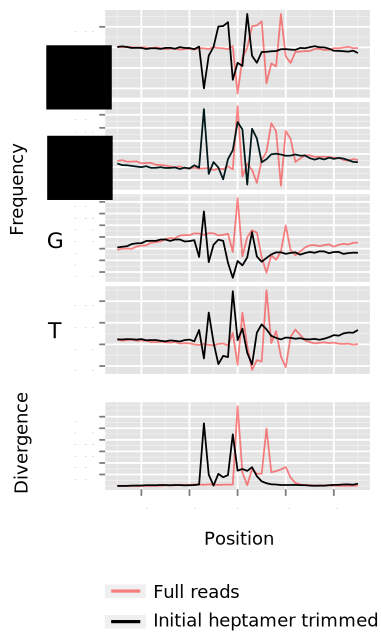
\includegraphics[width=0.35\textwidth]{fig/trimmed-freqs.pdf}
\end{center}
\caption{Nucleotide frequencies observed before (plotted in red) and after
(plotted in black) trimming the initial heptamer.}
\label{fig:trimmedfreqs}
\end{figure}


\section{Sensitivity of Parameters}

The performance of our method is dependent on two parameters: the standard
deviation at which background sequences are sampled, and the degree to which
model complexity in penalized. We have also introduced parameters limiting the
number of parents a node may have ($p_{\text{max}}$) as well as the distance
that an edge may traverse ($d_{\text{max}}$), but these exist only to control
the amount of CPU time used and have a much simpler interpretation: bigger is
better, but slower.

Here we retrain the model on 50,000 reads from the Mortazavi data
set, varying these first two parameters to assess the sensitivity of the
observed results to their values.

\begin{figure}[H]
\begin{center}
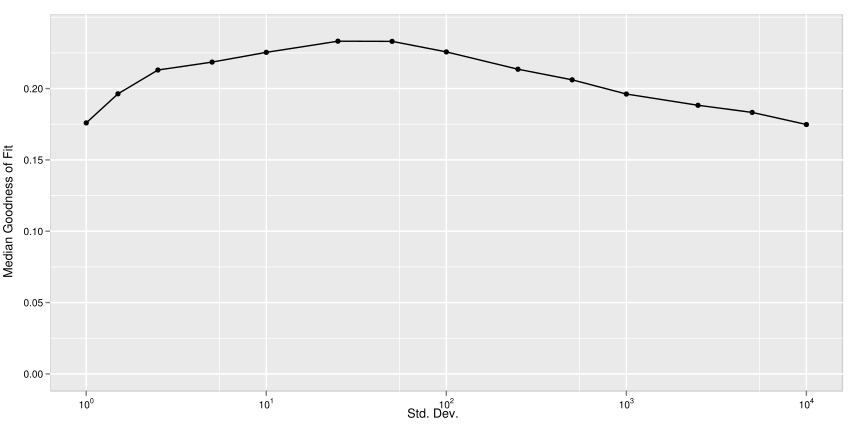
\includegraphics[width=0.8\textwidth]{fig/pois-sampstd.pdf}
\end{center}
\caption{Sensitivity of the parameter control he standard deviation at which
background sequences are sampled.}
\label{fig:poissampstd}
\end{figure}

Figure \ref{fig:poissampstd} show the standard deviation used to draw background
samples varied from 1 to 10,000. Apparent from this plot is that, while the
optimal choice lies somewhere between 10 and 100, the model performs
competitively for any reasonable value.


\begin{figure}[H]
\begin{center}
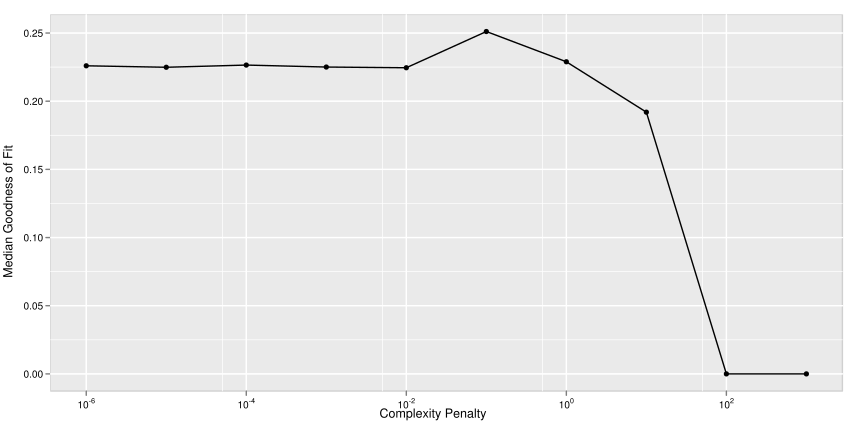
\includegraphics[width=0.8\textwidth]{fig/pois-comppen.pdf}
\end{center}
\caption{Sensitivity over adjustments to the complexity penalty.}
\label{fig:poiscomppen}
\end{figure}

Next we multiplied the complexity penalty term of the BIC by a constants varying
from $10^{-6}$ to $10^{3}$. (Recall that the BIC is $2\ell - m \log n$ where
$\ell$ is the log-likelihood, $m$ is the number of parameters needed to specify
the model, and $n$ is the number of training examples. Here we compute $2 \ell -
c m \log n$, varying $c$.)

It is clear from Figure \ref{fig:poiscomppen}, that a very severe complexity
penalty will result in a poor model. Here, for constants larger than 100, an
empty model is trained, resulting in a median $R^2$ of 0. Conversely, if
this constant is very small, a overly-dense model will be trained.  In this
data, for constants less than 0.01, the maximally dense model is trained (given
the restraints on in-degree and edge distance). This result is a sub-optimal but
entirely adequate solution.


\section{Additional Kullback-Leibler Divergence Plots}

Figure \ref{fig:klall} plots the adjusted and unadjusted KL divergence plots,
supplementing those in the results section of the main paper.

\begin{figure}[H]
\centerline{
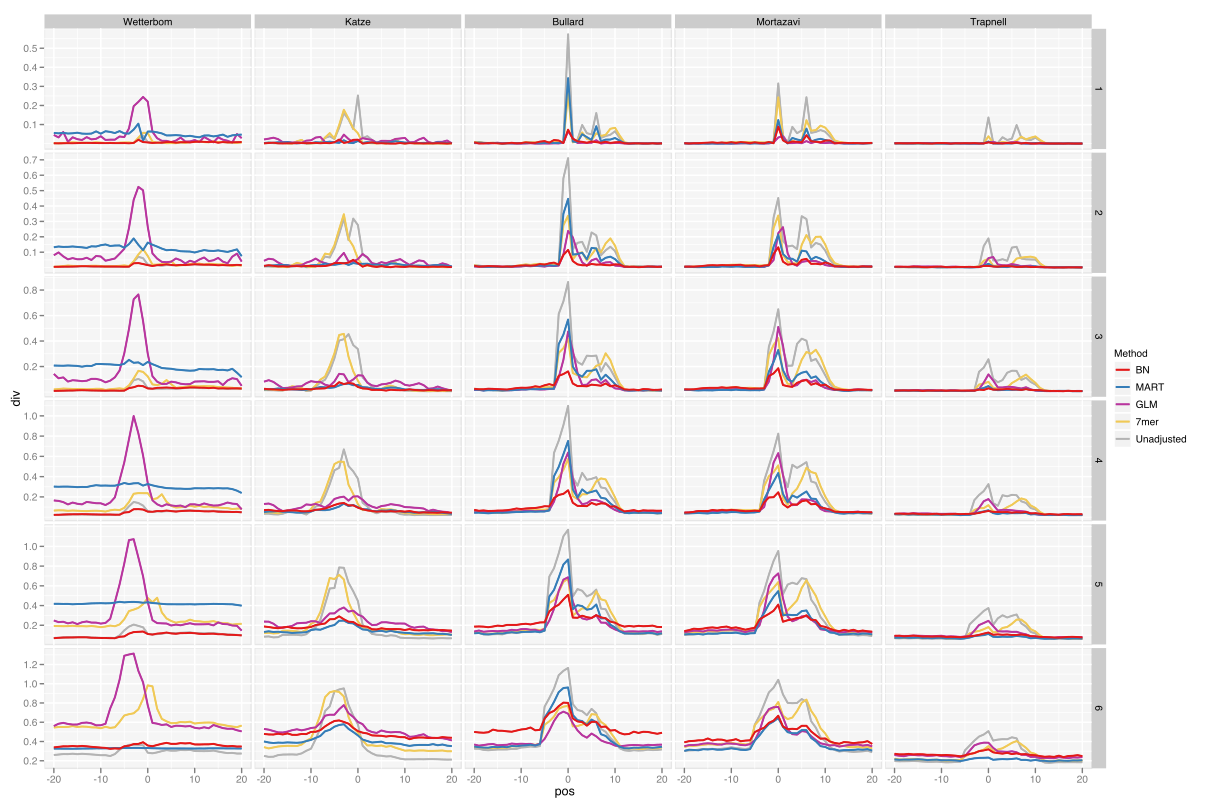
\includegraphics[width=\textwidth]{fig/kl-all.pdf}
}
\caption{}
\label{fig:klall}
\end{figure}


\section{Sequence bias in data from Au, et al., 2010}

Figure \ref{fig:aufreqs} plots sequence bias and KL divergence in the data
published by Au, et al. \cite{Au2010} and examined by us in Section 3.3.

\begin{figure}[H]
\centerline{\includegraphics[width=0.6\textwidth]{fig/au-freqs.pdf}}
\caption{}
\label{fig:aufreqs}
\end{figure}


\section{Runtime-Accuracy Trade-off}

Training our model on more reads results in more accurate estimation of bias,
but a longer training time. Here we investigate that trade-off by training our
model on progressively more reads from the Mortazavi data set. For each subset
we train our method, evaluate the median pseudo-coefficient of determination
($R^2$) over exons selected for our test set, and record the training time
required on one core of a 3Ghz Intel Xeon processor. These results are plotted
in Figure \ref{fig:poisn}.

\begin{figure}[H]
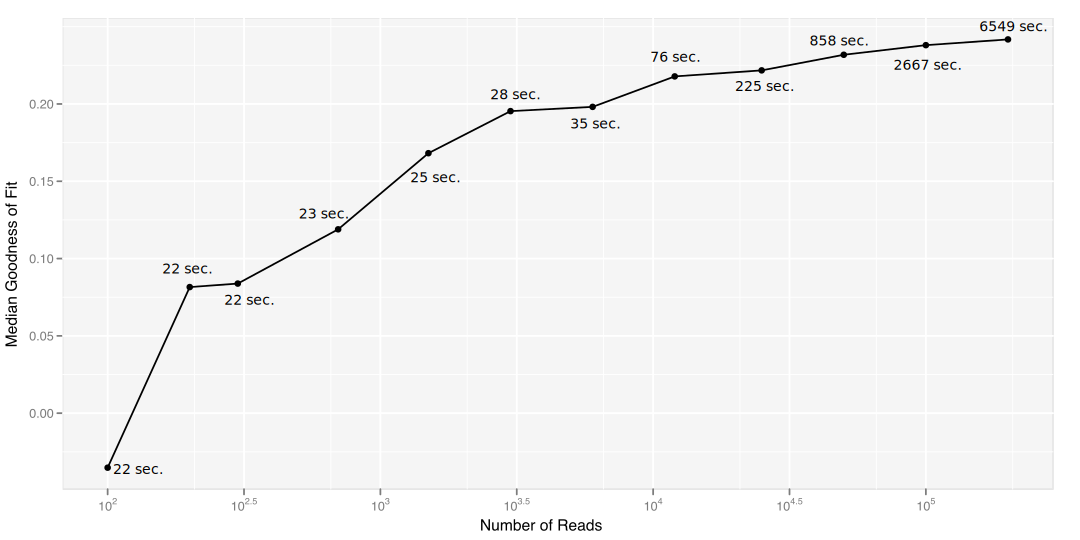
\includegraphics[width=\textwidth]{fig/pois-n.eps}
\caption{Median $R^2$ is plotted against training set size. Each point is
additionally labeled with the run time of the training procedure.}
\label{fig:poisn}
\end{figure}


%% TODO: coptions/labels below this point

\section{ChIP-Seq}

Though the MART model \cite{Li2010} performed very well in several cases, ours
offers the advantage that no gene annotations are required for training.  In
RNA-Seq this is useful in applications of de-novo gene discovery, but it also
allows our method to be applied to ChIP-Seq and other short read data. Here we
examine one publicly available ChIP-Seq data set from Cao, et. al.
\cite{Cao2010}. Specifically, we used one run, with Sequence Read Archive
accession number SRR034831, containing 3,873,192 reads. These were mapped to the
reference genome using Bowtie \cite{Langmead2009}, resulting in 1,382,867
uniquely mapped reads, which were used for this analysis.

Measuring nucleotide frequencies, we find the bias to be significantly less
than that observed the RNA-Seq data sets we tested, but the data was by no means
unbiased.

\begin{figure}[H]
\begin{center}
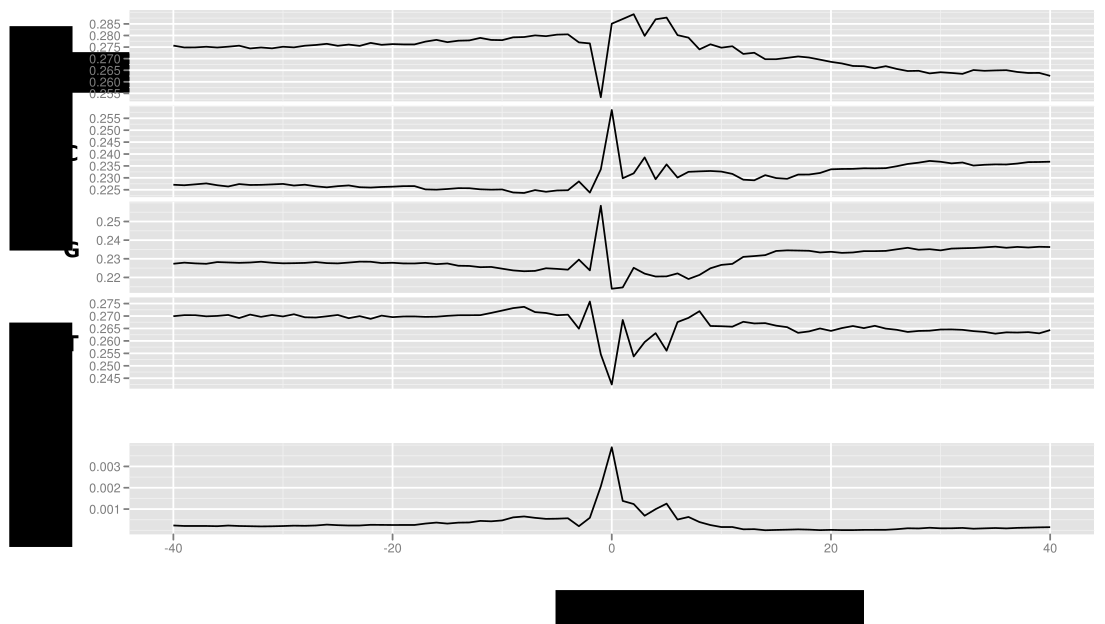
\includegraphics[width=0.7\textwidth]{fig/freqs_cao.pdf}
\end{center}
% TODO: caption
\label{fig:trimmedfreqs}
\end{figure}

In the analysis of the RNA-Seq data, we used the assumption of continuous
transcription across annotated exons to evaluate the efficacy of the models, as
well as to train the GLM and MART models. Evaluating bias correction on ChIP-Seq
data necessitates dropping the Poisson regression test, as well as the GLM and
MART models from our comparison, which can not be applied to such data.

We did however repeat our analysis using the Kullback-Leibler divergence.
We used several variations of the method described by Hansen, et. al.,
\cite{Hansen2010}. ``7mer'' estimated the initial heptamer, ``Avg-7mer''
averages the initial two heptamers, and ``4mer'' averages the initial two 4mers.

We trained each method using reads from chromosomes 1--8. The
remaining chromosomes were segmented into 500nt bins, and the KL divergence was
sampled from the 50,000 segments with the highest read counts.

Below, we plot directly the positional KL divergence, computed in tho same
manner described in the Results section of the paper.

\begin{figure}[H]
\begin{center}
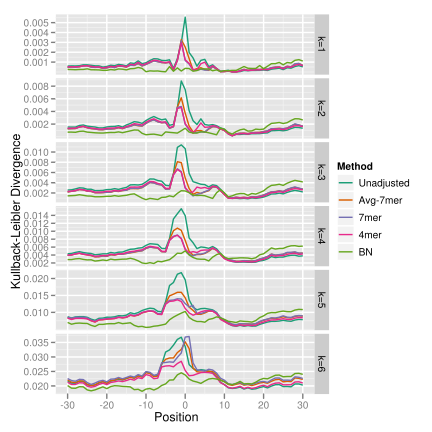
\includegraphics[width=0.5\textwidth]{fig/cao-kl.pdf}
\end{center}
% TODO: caption
\label{fig:trimmedfreqs}
\end{figure}

We see that our method is effective at reducing the bias in this ChIP-Seq data.



\section{Bias in Amplification-Free Sequencing}

To evaluate the extent to which the observed bias is caused by PCR amplification
in the library preparation stage, we analyzed data from the FRT-Seq protocol
developed by Mamanova, et. al. \cite{Mamanova2010}. FRT-Seq avoids the
amplification step during library preparation with reverse transcription
occuring on the flowcell surface. We obtained data generated by Mamanova, et.
al., from the European Nucleotide Archive with accession code ERR007689, and
mapped them to the hg19 assembly of the human genome with Bowtie
\cite{Langmead2009}. The nucleotide frequencies and divergence are plotted
below.

\begin{figure}[H]
\begin{center}
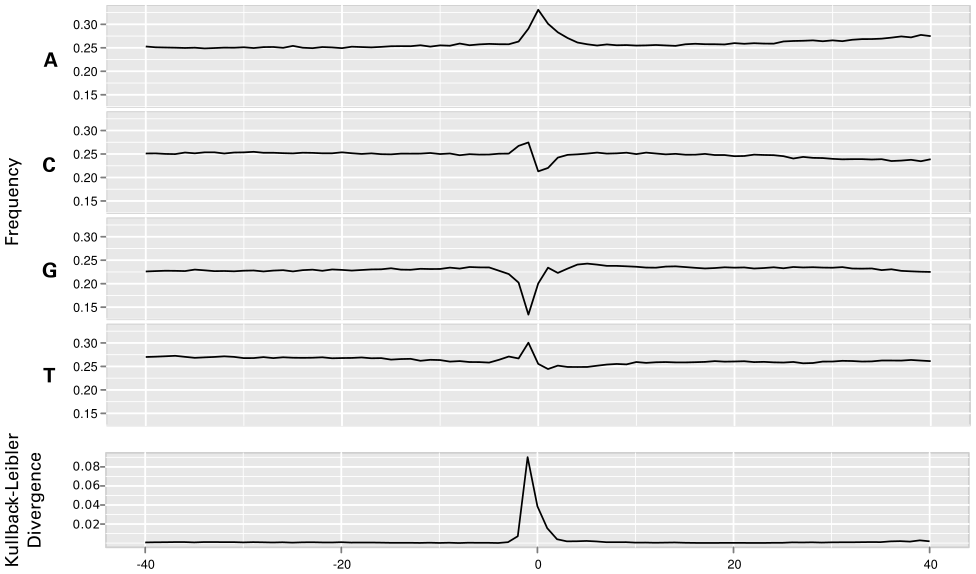
\includegraphics[width=0.6\textwidth]{fig/frt-all.pdf}
\end{center}
% TODO: caption
\label{fig:trimmedfreqs}
\end{figure}

It is clear from this analysis that the FRT-Seq method, as implemented to
generate this data, is not without bias, yet there is significant divergence at
only a small number of positions surrounding the read start. When our method is
trained on this data we obtain the suitably sparse model pictured below.

\begin{figure}[H]
\begin{center}
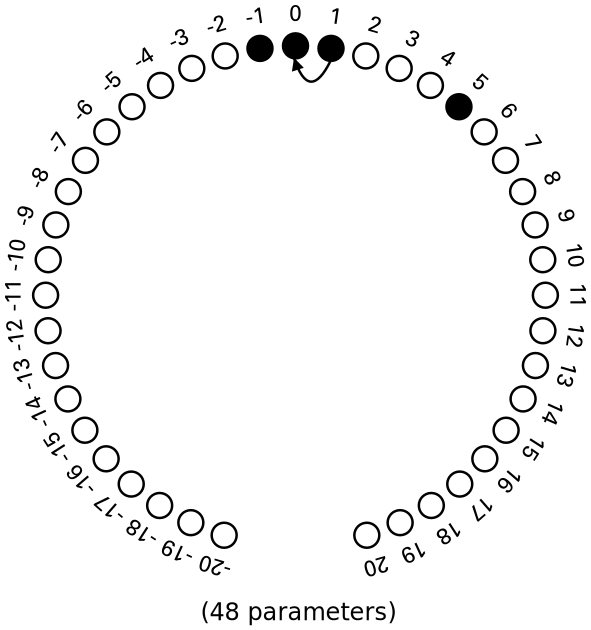
\includegraphics[width=0.4\textwidth]{fig/frt-graph.pdf}
\end{center}
% TODO: caption
\label{fig:trimmedfreqs}
\end{figure}


\section{Variability Between Replicates}

Measuring differential expression or isoform switching is a primary application of
RNA-Seq. If the bias were inconsistent between replicates, it would call into
question the accuracy of such tests. In our experiments, we have observed the
bias to be mostly, but not entirely consistent between replicates. Below, we
plot the frequencies from the four runs in the Trapnell data set.

\begin{figure}[H]
\begin{center}
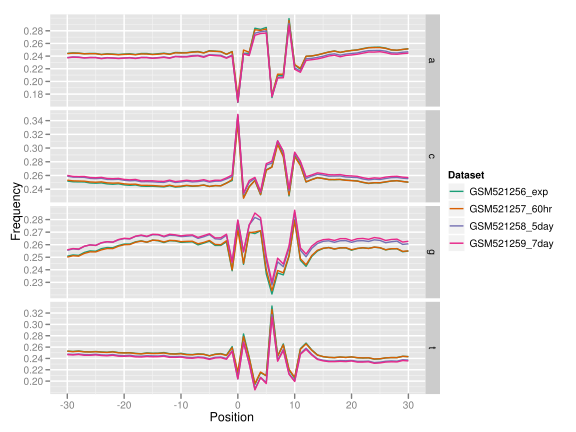
\includegraphics[width=0.7\textwidth]{fig/replicates.pdf}
\end{center}
% TODO: caption
\label{fig:trimmedfreqs}
\end{figure}

Though we do not know if the variability is always minor, assuming this is so,
there remains the risk that the sequence bias would greatly effect the depth to
which a locus is sequenced, and thus the statistical significance of
differential expression tests. This would bias the discovery of differentially
expressed genes, but not the test itself.


\section{KL Divergence}

\subsection{TODO: Title}

Suppose $P$ and $Q$ are probability distributions defined on a discrete sample
space. E.g., in the context of this paper, think of them as the probabilities of
DNA $k$-mers for some fixed $k$. The \emph{Kullback-Leibler divergence}, also
known as \emph{relative entropy}, of $Q$ with respect to $P$ is defined as
$$H(Q||P) = \sum_{i} q_i \ln \frac{q_{i}}{p_{i}}$$
where $q_{i}$ ($p_{i}$) is the probability of observing the i$^{\text{th}}$
event according to the distribution $Q$ (resp., $P$), and the summation is taken
over all events in the sample space (e.g., all $k$-mers). In some sense, this is
a measure of the dissimilarity between the distributions: if $p_{i} \approx
q_{i}$ everywhere, their log rations will be near zero and $H$ will be small; as
$q_{i}$ and $p_{i}$ diverge, their log rotions will deviate from zero and $H$
will increase.

For a more quantitative and (perhaps) intuitive interpretation, consider the
following hypothesis-testing scenario. Given $m$ independent samples from either
$P$ (arbitrarily called the ``null'') or from $Q$ (the ``alternative''), how
large should $m$ be to cenfidently choose between these cases? A natural
approach is to use a likelihood ratio test: letting $Y_i$ be the number of times
event $i$ is observed in $m$ trials ($\sum Y_i = m$), the likelihood of the
sequence of observations under model $P$ is $$\prod_{i} p_{i}^{Y_{i}}$$
and similarily for $Q$. So, the logarithm of the likelihood ratios is
$$
\text{LLR} =
\ln \frac{\prod_{i} q_{i} ^ {Y_{i}}}{\prod_{i} p_{i} ^ {Y_{i}}}
= \sum_{i} Y_{i} \ln \frac{q_{i}}{p_{i}}
= m \sum_{i} \frac{Y_{i}}{m} \ln \frac{q_{i}}{p_{i}} $$

If the sample is drawn from the alternative distribution $Q$, then the
expectation of $frac{Y_{i}}{m}$ is $q_i$, so the expected value of the LLR is
$$ m \sum_{i} q_{i} \ln \frac{q_{i}}{p_{i}} = m H(Q || P) $$
That is, the KL divergence is exactly the expected per-sample contribution to
the log-likelihood ratio.
%% when comparing these two hypotheses ??
So, assuming the null hypothesis is false, in order for it to be rejected with
$1000:1$ odds, one should choose $m$ to be inversely proportional to $H(Q ||
P)$:
\begin{align*}
m H(Q||P) \ge \ln 1000 \\
m \ge \frac{\ln 1000}{H(Q || P)}
\end{align*}

As a concrete example, all of the RNA-Seq data sets examined in this paper show
a KL divergence between the 1$^{\text{st}}$ positon of reads versus the
transcriptomic background nucleotide distribution of $0.05$ or greater. Thus,
one can confidently reject the hypothesis that reads are beeing uniformly
sampled across the transcriptome by examining only a few hundred randomly
selected reads (i.e., $\ln 1000 / 0.05 \approx 140$).


\subsection{Accuracy of Multinomial Parameter Estimation}

Continuing the notation above, suppose $P$ as an unknown distribution with
parameters $p_1, \dots, p_r$, $\sum p_i = 1$ where $r$ is the number of points
in the sample space (e.g. $r = 4^{k}$ in the case of $k$-mers). Given a random
ample $X_1, X_2, \dots, X_r$ of size $n = \sum_{i} X_i$ from $P$, it is well
known that the maximum likelihood estimators for the parameters are $q_i =
\frac{X_i}{n} \approx p_i$. How good an estimate for $P$ is this distribution
$Q$?

$$E[q_i] = E\left[\frac{X_i}{n}\right] = \frac{E[X_i]}{n} = \frac{np_i}{n} =
p_i$$
And the standard deviation of each estimate is proportional to $1/\sqrt{n}$. So
these estimates are increasingly accurate as the sample size increases. A more
quantitative assessment of the accuracy of the estimator is obtained by
evaluating the KL divergence:
$$H(Q||P)
= \sum_{i = 1}^{r} q_i \ln \frac{q_i}{p_i}
= \sum_{i = 1}^{r} q_i \ln \left(1 + \frac{q_i - p_i}{p_i} \right) $$
Using the first two terms of he Taylor series for $\ln (1 + x)$, this is
\begin{align*}
H(Q||P) &\approx \sum_{i = 1}^{r} q_i \left( \frac{q_i - p_i}{p_i} -
\frac{1}{2} \left( \frac{q_i - p_i}{p_i} \right)^2 \right ) \\
&= \sum_{i = 1}^{r} q_i \frac{q_i - p_i}{p_i} -
\frac{q_i}{2 p_i} \frac{(q_i - p_i)^2} {p_i}
\end{align*}
Since $\sum_{i = 1}^{r} q_i = \sum_{i = 1}^{r} pi = 1$,
$\sum_{i = 1}^{r} p_i \frac{q_i - p_i}{p_i} = 0$, so
\begin{align*}
H(Q||P) &\approx \sum_{i=1}^{r} q_i \frac{q_i - p_i}{p_i} - p_i \frac{q_i -
p_i}{p_i} - \frac{q_i}{2 p_i} \frac{(q_i - p_i)^2}{p_i} \\
&= \sum_{i=1}^{r} \frac{(q_i - p_i)^2}{p_i}\left(1 - \frac{q_i}{2 p_i}\right) \\
&\approx \frac{1}{2} \sum_{i=1}^{r} \frac{(q_i - p_i)^2}{p_i}
\end{align*}
since $q_i \approx p_i$. Multiplying by $n^2 / n^2$ we have,
\begin{align*}
H(Q||P) &\approx \frac{1}{2n} \sum_{i=1}^{r} \frac{n q_i - n p_i)^2}{n p_i} \\
        &= \frac{1}{2n} \sum_{i=1}^{r} \frac{(X_i - E[X_i])^2}{E[X_i]}
\end{align*}

The summation is the test statistic for the $\chi^2$ goodness-of-fit test for a
multinomial distribution, and as $n \rightarrow \infty$ is known to follow a
$\chi^2$ distribution with $r - 1$ degrees of freedom. Finally, the expected
value of such a random variable is $r - 1$, hence the expected KL divergence of
the MLE inferred distribution $Q$ with respect to the true distribution $P$ is
\begin{equation}
\label{eq:entropy}
E[H(Q||P)] = \frac{r - 1}{2n}
\end{equation}

Stochastic simulations of this proves when $P$ is uniform show that the above
formula is a very good fit when $n > r$.

\begin{figure}[H]
\centerline{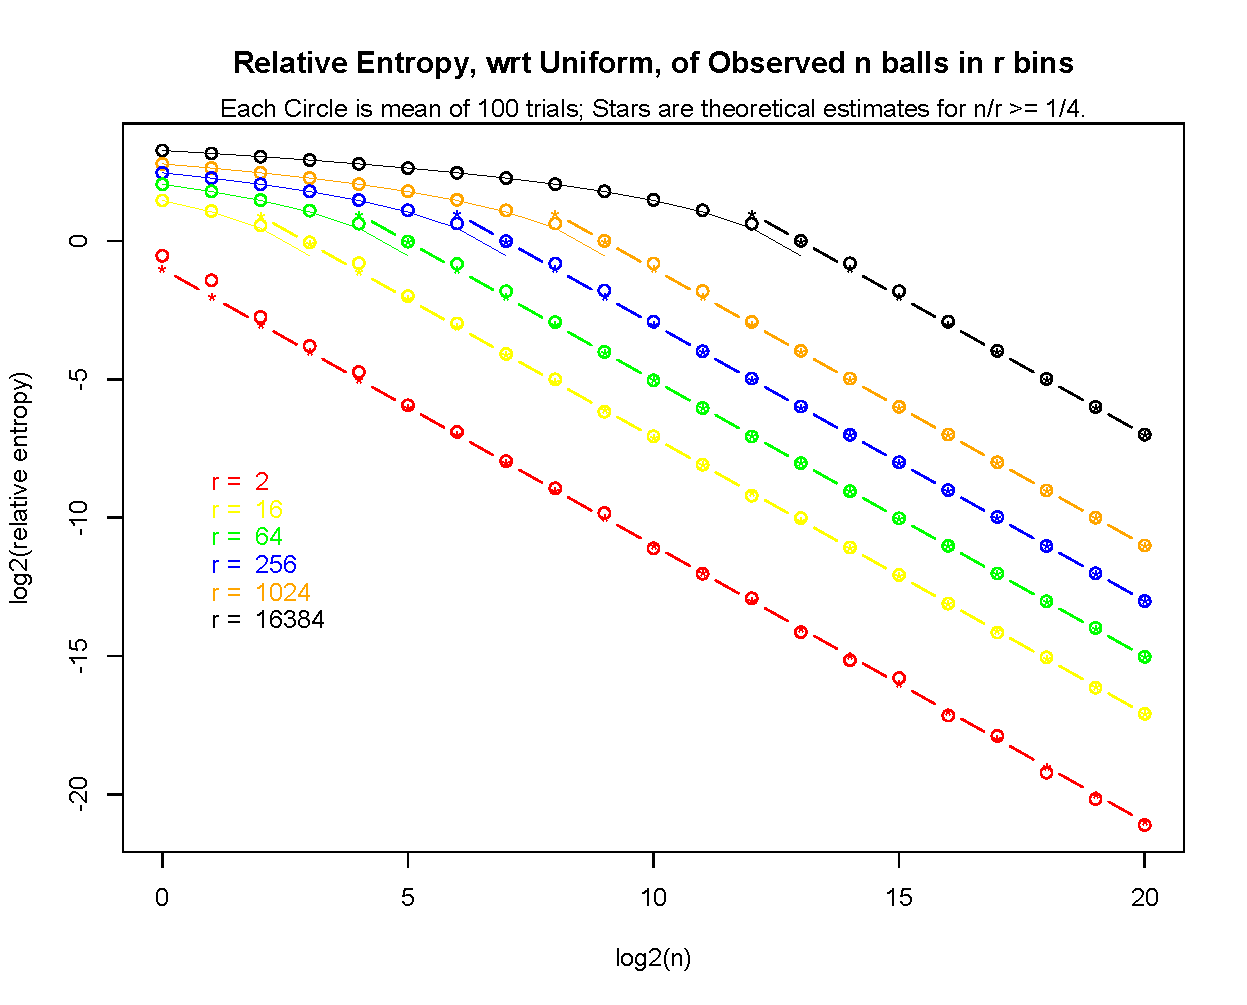
\includegraphics[width=0.8\textwidth]{fig/entropy.pdf}}
\caption{For each value of $n$ plotted, the circles indicate the value of
$H(Q||P)$, averaged over 100 samples of size $n$, where $P$ is uniform and $Q$
is the MLE estimator for $P$ basen on $n$ random samples drawn from $r$ bins.
The asterisks and the straight line interpolating them are the theoretical
approximation from Equation \ref{eq:entropy}.
}
\label{fig:entropy}
\end{figure}

\bibliographystyle{plain}
\bibliography{seqbias-paper}

\end{document}




